\documentclass{article}
\usepackage[portuguese]{babel}
\usepackage[square,numbers]{natbib}
\bibliographystyle{abbrvnat}
\usepackage{url}
\usepackage{pdfpages}
\usepackage[table,xcdraw]{xcolor}
\usepackage{amsmath}
\usepackage{graphicx}
\usepackage{listingsutf8}
\graphicspath{{images/}}
\usepackage{parskip}
\usepackage{fancyhdr}
\usepackage{vmargin}
\usepackage{float}
\usepackage{caption}
\usepackage{subcaption}
\usepackage{hyperref}
\usepackage{listings}
\usepackage{pdfpages}
\usepackage{bytefield}
\usepackage{array} 
\usepackage{xparse}
\usepackage{tikz}
\usepackage{verbatim}
\usepackage{arydshln}
\usepackage{mathtools}
\usepackage{booktabs}
\usepackage{tabulary,lipsum}
\usepackage{svg}
\usepackage{pdflscape}
\usepackage{minted}

\usepackage{fancyhdr}
\pagestyle{fancy}

\tymin=60pt
\tymax=\maxdimen

\setminted{
fontsize=\large,
breaklines,
breakbytoken=false,
breakautoindent=true,
baselinestretch=1.0,
framesep=2mm,
numbersep=2mm,
linenos,
frame=leftline
}

\renewcommand{\theFancyVerbLine}{\sffamily \textcolor[rgb]{0,0,0}{\large {\arabic{FancyVerbLine}}}}


\newcommand{\sectionbreak}{\clearpage}


\newcommand{\tikzb}[1]{\newsavebox{\#1}}

\setmarginsrb{3 cm}{2.5 cm}{3 cm}{2.5 cm}{1 cm}{1.5 cm}{1 cm}{1.5 cm}


\setlength\parindent{24pt}


\NewDocumentCommand{\codeword}{v}{%
\texttt{\textcolor{codegreen}{#1}}%
}

\usepackage[framed,numbered]{matlab-prettifier}
\lstset{
  style      = Matlab-editor,
  basicstyle = \fontfamily{pcr}\selectfont\footnotesize, % if you want to use Courier
}

\lstdefinelanguage{C2}[]{C}{
    %morestring = [s][\color{codelaranja}]{  <}{>},
}

\lstdefinestyle{mystyle}{
    backgroundcolor=\color{backcolour},   
    commentstyle=\color{codegreen},
    keywordstyle=\color{AzulTop},
    numberstyle=\tiny\color{codegray},
    stringstyle=\color{codelaranja},
    basicstyle=\ttfamily\footnotesize,
    breakatwhitespace=false,         
    breaklines=true,                 
    captionpos=b,                    
    keepspaces=true,                 
    numbers=left,                    
    numbersep=5pt,                  
    showspaces=false,                
    showstringspaces=false,
    showtabs=false,                  
    tabsize=2,
}

\definecolor{codegreen}{rgb}{0,0.6,0}
\definecolor{codegray}{rgb}{0.5,0.5,0.5}
\definecolor{codelaranja}{rgb}{0.93,0.6,0.32}
\definecolor{backcolour}{rgb}{0.95,0.95,0.92}
\definecolor{AzulTop}{rgb}{0.3,0.55,0.94}
\definecolor{LightCyan}{rgb}{0.88,1,1}


\lstset{
    style=mystyle, 
    inputencoding=utf8,
    extendedchars=true,
    literate={á}{{\'a}}1 {à}{{\`a}}1 {ã}{{\~a}}1  {Ã}{{\~A}}1 {â}{{\^a}}1 {é}{{\'e}}1 {ê}{{\^e}}1 {ë}{{\"e}}1 {í}{{\'i}}1 {ç}{{\c{c}}}1 {Ç}{{\c{C}}}1 {õ}{{\~o}}1 {ó}{{\'o}}1 {ô}{{\^o}}1 {ú}{{\'u}}1
}


\title{Relatório do Laboratório 4}								% Title
\author{} %<------------------------------------------------------								% Author
\date{\today}											% Date

\makeatletter
\let\thetitle\@title
\let\theauthor\@author
\let\thedate\@date
\makeatother

\pagestyle{fancy}
\fancyhf{}
\rhead{\theauthor}
\lhead{\thetitle}
\cfoot{\thepage}


\ifpdf
  \DeclareGraphicsRule{*}{mps}{*}{}
\fi




\begin{document}

%%%%%%%%%%%%%%%%%%%%%%%%%%%%%%%%%%%%%%%%%%%%%%%%%%%%%%%%%%%%%%%%%%%%%%%%%%%%%%%%%%%%%%%%%

\begin{titlepage}
	\centering
    \vspace*{0.2 cm}
    
\includegraphics[scale = 0.8]{logoPoli.jpg}\\[1.0 cm]	% University Logo
    \textsc{\LARGE \newline\newline Escola Politécnica da USP}\\[1.5 cm]	% University Name
    \textsc{\Large PMR3406 - Microprocessadores em Automação e Robótica}\\[0.5 cm] %Course Code     
    \textsc{\Large Turma 03 - Grupo 02}\\[0.5 cm]
	
	\rule{\linewidth}{0.2 mm} \\[0.4 cm]
	{ \huge \bfseries \thetitle}\\ 
	\rule{\linewidth}{0.2 mm} \\[1 cm]
	
	\begin{minipage}{0.5\textwidth}
		\begin{flushleft} \large

                Antônio Augusto Carnevalli\\
                Thiago Lam Braweman\\
			
			\end{flushleft}
	\end{minipage}~
	\begin{minipage}{0.5\textwidth}
            
		\begin{flushright} \large
			
                13682909\\
                10770502\\
		    
		    \end{flushright}
        
	\end{minipage}\\~
	\vfill
	\thedate
	
    
\end{titlepage}

\
%-------------------------------------------------------------
\section{Cálculos do Timer 0}

%-------------------------------------------------------------
%                             ATENÇÃO!!!! REVER TUDO
%------------------------------------------------------------



Para essa atividade precisamos fazer 4 leituras com o sensor de proximidade por segundo, para isso usaremos a interrupção gerada pelo timer 0 para controlar a frequência dessas medições. Conforme a primeira página do datasheet \cite{PICDatasheet}, o PIC16F886 possui uma frequência de operação $F_{OSC}$ de 20 MHz, ou seja, o período do clock interno $4/F_{OSC}$ é igual a 200 ns.\par

Antes de realizar 4 leituras em 1 segundo precisamos ajustar o timer 0 para que a interrupção ocorra a cada 5 ms, o PIC utiliza um prescaler e o valor inicial do timer 0 para conseguirmos nos aproximar do tempo desejado.
O prescaler define o intervalo de tempo que o timer 0 vai ser chamado e o valor inicial quantas vezes ele deve ser chamado. A escolha desses não é aparente, então devemos calcular e achar o resultado que minimiza o erro para cada um dos prescalers, como o exemplo abaixo.\par

Temos que nossas condições iniciais são:

\begin{align*}
    &T_{interno} = 200 ns\\
    &T_{desejado} = 5 ms
\end{align*}

Escolhendo um valor para o prescaler achamos o valor do período em que o timer 0 é chamado.
\begin{align*}
   &T1 = T_{interno} * P_{scaler}\\
   &T1 = 200 * 128 = 25600 ns\\ 
   &T1=25,6\mu s
\end{align*}

Agora devemos calcular quantas vezes o timer 0 deve ser chamado para que o intervalo de tempo seja o mais próximo possível do desejado. (Lembrando que esse valor é um inteiro e não um float).

\begin{align*}
   &T0I = \dfrac{T_{desejado}}{T_{interno}* P_{scaler}}\\\\
   &T0I = \dfrac{5*10^{-3}}{200^{-6}*256} = 195,3125\\\\
   &T0I \approx 195
\end{align*}

Agora podemos calcular o período real que a interrupção ira acontecer, multiplicando T0I e T1.

\begin{align*}
   &T = T0I * T1\\
   &T = 195 * 25600 = 0,004992s
\end{align*}

Com esse valor definido podemos calcular o erro em relação o $T_{desejado}$.

\begin{align*}
   &Erro_\%= \dfrac{|T_{desejado}-T|}{T_{desejado}} * 100\\\\
   &Erro_\%= \dfrac{|5-4,992|}{5}*100\\\\
   &Erro_\%= 0,16\%
\end{align*}

Esse mesmo procedimento foi aplicado para cada um dos prescalers (Figura \ref{Tabel5ms}).

%--------------------------------------------------------
%                Tabela 1 de cálculo do T0
%--------------------------------------------------------

\begin{figure}[H]
\centering

\begin{tabular}{|c|c|c|c|c|c|c|}
\hline
\rowcolor[HTML]{FFD966} 
\cellcolor[HTML]{FFD966}\textbf{Fosc MHz} & \cellcolor[HTML]{FFD966}\textbf{Clock interno ns} & \cellcolor[HTML]{FFD966}\textbf{Prescaler} & \cellcolor[HTML]{FFD966}\textbf{T1 ns} & \cellcolor[HTML]{FFD966}\textbf{T0I} & \cellcolor[HTML]{FFD966}\textbf{T s} & \cellcolor[HTML]{FFD966}\textbf{Erro} \\ \hline
\rowcolor[HTML]{FFFFFF} 
20                                                          & 200                                                                & 2                   & 400                                                       & 255          & 0,000102                                               & 97,96\%       \\ \hline
\rowcolor[HTML]{FFFFFF} 
20                                                          & 200                                                                & 4                   & 800                                                       & 255          & 0,000204                                               & 95,92\%       \\ \hline
\rowcolor[HTML]{FFFFFF} 
20                                                          & 200                                                                & 8                   & 1.600                                                     & 255          & 0,000408                                               & 91,84\%       \\ \hline
\rowcolor[HTML]{FFFFFF} 
20                                                          & 200                                                                & 16                  & 3.200                                                     & 255          & 0,000816                                               & 83,68\%       \\ \hline
\rowcolor[HTML]{FFFFFF} 
20                                                          & 200                                                                & 32                  & 6.400                                                     & 255          & 0,001632                                               & 67,36\%       \\ \hline
\rowcolor[HTML]{FFFFFF} 
20                                                          & 200                                                                & 64                  & 12.800                                                    & 255          & 0,003264                                               & 34,72\%       \\ \hline
\rowcolor[HTML]{FFFFFF} 
20                                                          & 200                                                                & 128                 & 25.600                                                    & 195          & 0,004992                                               & 0,16\%        \\ \hline
\rowcolor[HTML]{FFFFFF} 
20                                                          & 200                                                                & 256                 & 51.200                                                    & 98           & 0,005018                                               & 0,35\%        \\ \hline
\end{tabular}

\caption{Tabela de resultados para o Timer 0.}
\label{Tabel5ms}

\end{figure}

Com a interrupção do timer 0 ocorrendo a aproximadamente 5 ms temos só que criar uma nova variável \textbf{m} que irá contar o número de vezes que o timer 0 é chamado para que as leituras ocorram a cada 0,25 s.\par

Assim para cada valor de prescaler determinamos o valor de m e seu respectivo erro (Figura \ref{Tabel250ms}).


%--------------------------------------------------------
%                Tabela 2 de cálculo do T0
%--------------------------------------------------------


\begin{figure}[H]
\begin{tabular}{|c|c|c|c|c|c|c|c|}
\hline
\rowcolor[HTML]{FFD966} 
\textbf{Fosc MHz} & \textbf{Clock interno ns} & \textbf{Prescaler} & \textbf{T1 ns} & \textbf{T0I} & \textbf{m} & \textbf{T s} & \textbf{Erro} \\ \hline
\rowcolor[HTML]{FFFFFF} 
20                & 200                       & 2                   & 400            & 255          & 2451        & 0,250        & 0,0008\%     \\ \hline
\rowcolor[HTML]{FFFFFF} 
20                & 200                       & 4                   & 800            & 255          & 1225       & 0,250        & 0,0400\%     \\ \hline
\rowcolor[HTML]{FFFFFF} 
20                & 200                       & 8                   & 1.600          & 255          & 613        & 0,250        & 0,0416\%     \\ \hline
\rowcolor[HTML]{FFFFFF} 
20                & 200                       & 16                  & 3.200          & 255          & 306        & 0,250        & 0,1216\%     \\ \hline
\rowcolor[HTML]{FFFFFF} 
20                & 200                       & 32                  & 6.400          & 255          & 153        & 0,250        & 0,1216\%      \\ \hline
\rowcolor[HTML]{FFFFFF} 
20                & 200                       & 64                  & 12.800         & 255          & 77         & 0,251        & 0,5312\%      \\ \hline
\rowcolor[HTML]{FFFFFF} 
20                & 200                       & 128                 & 25.600         & 195          & 50         & 0,250        & 0,1600\%      \\ \hline
\rowcolor[HTML]{FFFFFF} 
20                & 200                       & 256                 & 51.200         & 98           & 50         & 0,251        & 0,3520\%      \\ \hline
\end{tabular}
\iffalse
\begin{tabular}{|c|c|c|c|c|c|c|c|}
\hline
\rowcolor[HTML]{FFD966} 
\textbf{Fosc MHz} & \textbf{Clock interno ns} & \textbf{Pré-scaler} & \textbf{T1 ns} & \textbf{T0I} & \textbf{m} & \textbf{T s} & \textbf{Erro} \\ \hline
\rowcolor[HTML]{FFFFFF} 
20                & 200                       & 2                   & 400            & 255          & 2.451      & 0,250        & 0,0008\%      \\ \hline
\rowcolor[HTML]{FFFFFF} 
20                & 200                       & 4                   & 800            & 255          & 1.225      & 0,250        & 0,0400\%      \\ \hline
\rowcolor[HTML]{FFFFFF} 
20                & 200                       & 8                   & 1.600          & 255          & 613        & 0,250        & 0,0416\%      \\ \hline
\rowcolor[HTML]{FFFFFF} 
20                & 200                       & 16                  & 3.200          & 255          & 306        & 0,250        & 0,1216\%      \\ \hline
\rowcolor[HTML]{FFFFFF} 
20                & 200                       & 32                  & 6.400          & 255          & 153        & 0,250        & 0,1216\%      \\ \hline
\rowcolor[HTML]{FFFFFF} 
20                & 200                       & 64                  & 12.800         & 255          & 77         & 0,251        & 0,5312\%      \\ \hline
\rowcolor[HTML]{FFFFFF} 
20                & 200                       & 128                 & 25.600         & 195          & 50         & 0,250        & 0,1600\%      \\ \hline
\rowcolor[HTML]{FFFFFF} 
20                & 200                       & 256                 & 51.200         & 98           & 50         & 0,251        & 0,3520\%      \\ \hline
\end{tabular}
\fi
\caption{Tabela de resultados para o Timer 0 com a variável m.}
\label{Tabel250ms}
\end{figure}

Assim os resultados obtidos no final são:

\begin{align*}
    & P_{scaler} = 1:128\\
    & T0I = 195 \\
    & m = 50\\
\end{align*}

Podemos notar que outras opções de prescaler minimizam mais o erro no final, porém como outras partes do código podem usar o Timer 0 o seu erro tem prioridade. Além disso, o erro de 0,16\% já é adequado para nosso uso.
%-------------------------------------------------------------
\section{ Inicialização e utilização do canal de conversão A/D}


% Explicação sobre como inicializar e utilizar um canal de conversão A/D do PIC com base
% no estudo do data sheet do PIC 16F886 e do código da biblioteca adc.c. Mostre e explique
% todos os bits que devem ser programados para tanto.

\subsection{Fontes de consulta}

O PIC que utilizamos nessa disciplina é o PIC16F886 com 28 pinos (Figura \ref{PICpins}) baseado na apostila da disciplina \cite{Apostila}, para iniciar e utilizar a conversão A/D temos como referência o diagrama de pinos do PIC (Figura \ref{PICpins}), o diagrama de blocos do módulo de conversão A/D (Figura \ref{ADCBlock}) (riscados em vermelho os canais inexistentes no nosso modelo), e a tabela dos registradores do ADC, retirados das páginas 3, 103 e 113 do datasheet \cite{PICDatasheet}.\par

\begin{figure}[H]
    \centering
    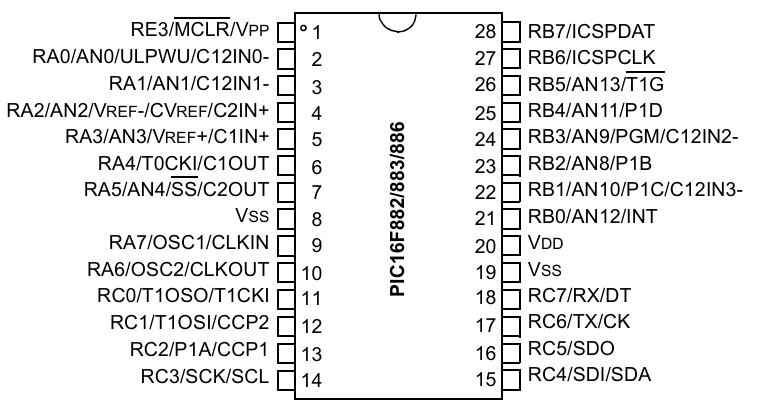
\includegraphics[ width = 0.8\linewidth]{images/PIC16F886pins.png}
    \caption{Diagrama de pinos do PIC16F886 (28 pinos)}
    \label{PICpins}
\end{figure}

\begin{figure}[H]
    \centering
    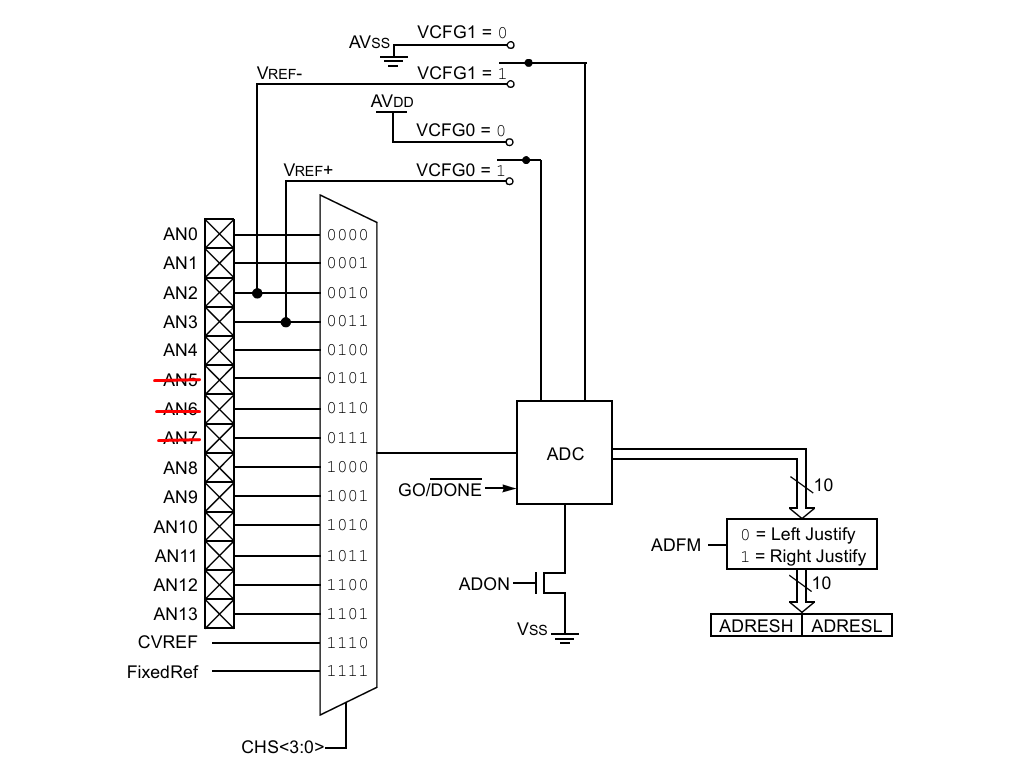
\includegraphics[ width = 0.8\linewidth]{images/ADCBlockDiagram.png}
    \caption{Diagrama de blocos do módulo ADC do PIC.}
    \label{ADCBlock}
\end{figure}

\begin{figure}[H]
    \centering
    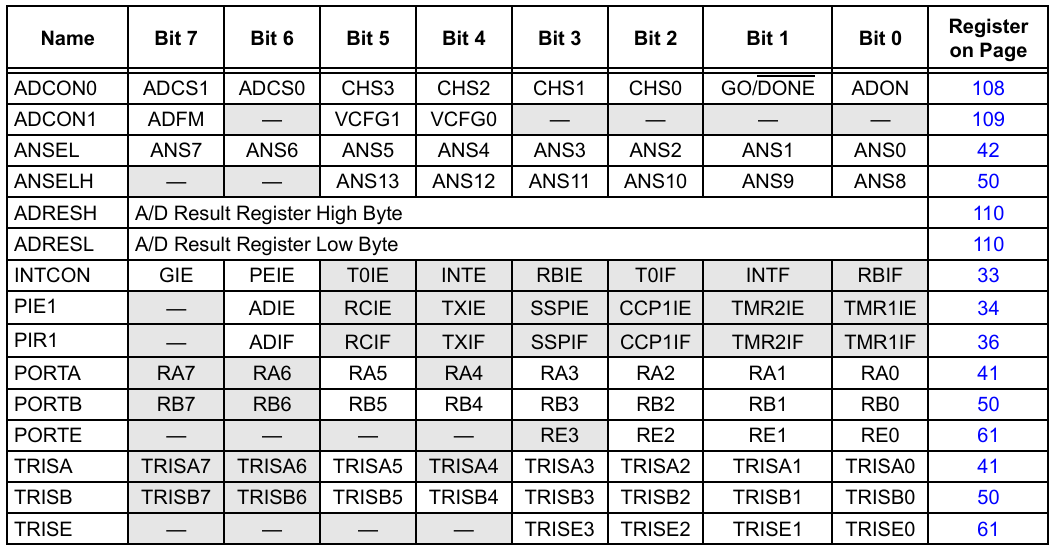
\includegraphics[ width = 0.8\linewidth]{images/ADCRegisters.png}
    \caption{Resumo dos Registradores utilizados pelo conversor A/D.}
    \label{ADCRegisters}
\end{figure}

\subsection{Inicialização do conversor}

Antes de iniciar o processo de conversão temos que configurar certos bits reservados, temos que escolher o canal do ADC que vamos utilizar, como visto no diagrama de blocos (Figura \ref{ADCBlock}) temos 11 canais disponíveis, \textbf{AN0-AN4} e \textbf{AN8-AN13}. Para realizar essa decisão temos que alterar os 4 bits $CHS<3:0>$ do registrador ADCON0 (Figura \ref{ADCRegisters}), para que eles correspondam aos bits do canal escolhido (Figura \ref{ADCBlock}).\par

%-------------------------Pinos-----------------------------------------------
Escolhido o canal devemos ajustar os pinos que vamos utilizar, os pinos correspondentes a cada canal podem ser obtidos a partir do diagrama (Figura \ref{PICpins}) ou na tabela abaixo (Figura \ref{PINChannelTable}).\par

\begin{figure}[H]

\centering
\begin{tabular}{|c|c|c|}
\hline
\rowcolor[HTML]{FFD966} 
\textbf{Canal} & \textbf{Pino} & \textbf{N° do pino} \\ \hline
\rowcolor[HTML]{FFFFFF} 
\textbf{AN0}   & RA0           & 2                   \\ \hline
\rowcolor[HTML]{FFFFFF} 
\textbf{AN1}   & RA1           & 3                   \\ \hline
\rowcolor[HTML]{FFFFFF} 
\textbf{AN2}   & RA2           & 4                   \\ \hline
\rowcolor[HTML]{FFFFFF} 
\textbf{AN3}   & RA3           & 5                   \\ \hline
\rowcolor[HTML]{FFFFFF} 
\textbf{AN4}   & RA5           & 7                   \\ \hline
\rowcolor[HTML]{FFFFFF} 
\textbf{AN8}   & RB2           & 23                  \\ \hline
\rowcolor[HTML]{FFFFFF} 
\textbf{AN9}   & RB3           & 24                  \\ \hline
\rowcolor[HTML]{FFFFFF} 
\textbf{AN10}  & RB1           & 22                  \\ \hline
\textbf{AN11}  & RB4           & 25                  \\ \hline
\textbf{AN12}  & RB0           & 21                  \\ \hline
\textbf{AN13}  & RB5           & 26                  \\ \hline
\end{tabular}

\caption{Tabela da relação entre pinos e canais analógicos.}
\label{PINChannelTable}
\end{figure}

%----------------------------------Input------------------------------------
Existem 2 ajustes necessários com relação aos pinos, primeiro ele deve atuar como uma entrada, então nos registradores TRISx deve-se colocar 1 no bit correspondente ao pino escolhido.\par

%--------------------------------Entrada analógica------------------------------
O outro ajuste é no tipo de entrada, analógica ou digital, para o conversor A/D usamos entrada analógica, devemos então alterar no registrador ANSEL ou ANSELH o bit correspondente ao pino escolhido.\par

%----------------------------------Formato do resultado-----------------------------
A saída de um conversor A/D é um número em base 2 com n-bits, onde n é a resolução do resultado, no caso do PIC16F886 a resolução do conversor A/D é de 10-bits. Como os registradores têm 8-bits, são necessários dois registradores para a leitura dos resultados, eles são ADRESH para os bits mais significativos e ADRESL para os menos (Figura \ref{ADCRegisters}). Por conta do excesso de bits disponíveis, podemos escolher se esses serão justificados a direita ou a esquerda conforme a imagem abaixo (Figura \ref{ADCResult}) retirada da página 106 do datashet \cite{PICDatasheet}. 

    \begin{figure}[H]
        \centering
        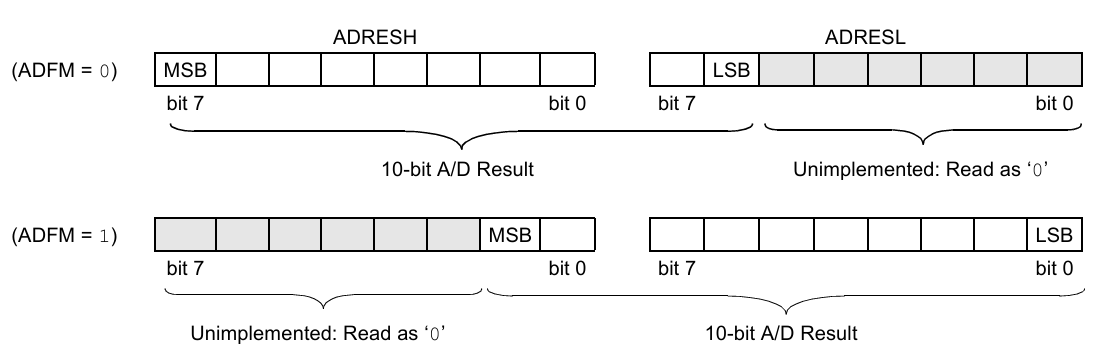
\includegraphics[ width = 0.8\linewidth]{images/ADCresult.png}
        \caption{Resultado da conversão A/D de 10 bits}
        \label{ADCResult}
    \end{figure}

Para fazer o ajuste devemos ajustar o bit ADFM do registrador ADCON1, igualando ele a 0 para justificar a esquerda e 0 para a direita assim (Figura \ref{ADCResult}).\par

%-----------------------------------Clock--------------------------------------
Outra parte da configuração é o ajuste do período do clock do módulo ADC, chamamos esse período de $T_{AD}$, esse valor representa o tempo de conversão de 1 bit, no caso do PIC o resultado com 10-bits leva por volta de 11 $T_{AD}$ (Figura \ref{ADCCycle}), retirado da página 105 do datasheet \cite{PICDatasheet} isso leva em consideração que o processo tem início aproximadamente 1 $T_{AD}$ depois da chamada. (Um ponto importante é que após o ciclo da conversão é necessário 2 $T_{AD}$ antes de realizar outra conversão).\par

    \begin{figure}[H]
        \centering
        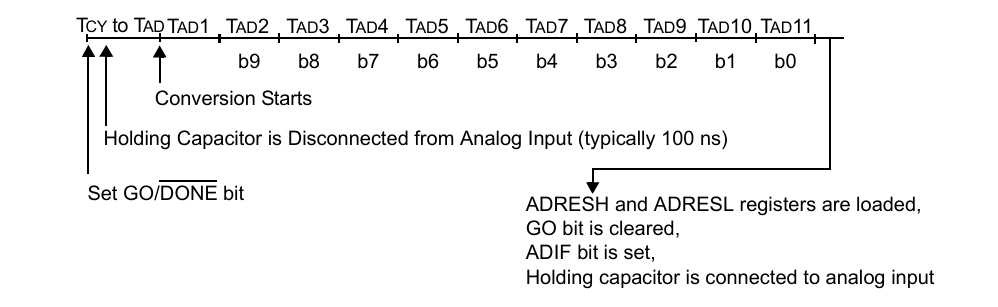
\includegraphics[ width = 0.8\linewidth]{images/ADCCycles.png}
        \caption{Ciclo da conversão A/D no PIC.}
        \label{ADCCycle}
    \end{figure}

Valores aceitáveis para $T_{AD}$ estão entre $1,6\mu s$ e $6\mu s$ e para conseguirmos chegar neles devemos alterar os bits $ADCS<1:0>$ do registrador ADCON0 (Figura \ref{TADTable}), retirada da página 105 do datasheet \cite{PICDatasheet}.\par

    \begin{figure}[H]
        \centering
        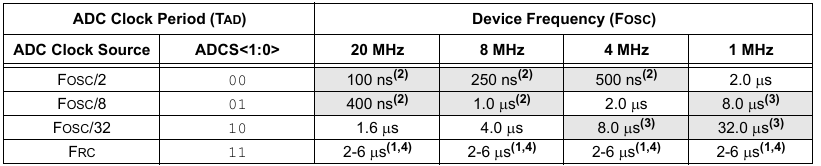
\includegraphics[ width = 0.8\linewidth]{images/TabelaTAD.png}
        \caption{Tabela do período do clock $T_{AD}$ por frequência de operação $F_{OSC}$}
        \label{TADTable}
    \end{figure}

Como a frequência do oscilador do dispositivo ($F_{OSC}$) é de 20MHz, temos que a única opção aceitável para os bits $ADCS<1:0>$ é de $0b10$, para que $T_{AD}$ seja $32/F_{OSC}$ ou $1,6\mu s$, ficando por tanto dentro da margem.\par

%---------------------------Tensão de Referência--------------------------------
O resultado da conversão, como mencionado anteriormente, é um número binário com 10 bits, porém seu valor depende das tensões de referência $V_{Ref}^+$ (Referência superior da tensão) e $V_{Ref}^-$ (Referência inferior da tensão), ou seja, o menor resultado possível 0b0000000000 equivale a tensão $V_{Ref}^-$ e o maior 0b1111111111 equivale a tensão $V_{Ref}^+$.\par

Os valores de referência, por padrão, equivalem a alimentação do microcontrolador ($V_{DD}$) como referência superior, e o terra dele ($V_{SS}$) a referência inferior. Porém, podemos alterar esses valores usando os bits $VCFG<1:0>$ do registrador ADCON1.\par

Conforme vimos no diagrama de blocos (Figura \ref{ADCBlock}) o bit $VCFG0$ permite mudar o valor de $V_{Ref}^+$ para o valor que está sendo lido na entrada do canal AN3 (pino RA3), da mesma forma, o bit $VCFG1$ permite mudar o valor de $V_{Ref}^-$ para o valor que está sendo lido na entrada do canal AN2 (pino RA2).\par

%------------------------------Interrupção---------------------------------
O módulo ADC do PIC que utilizamos oferece a opção de criar interrupções, para habilitar isso o bit ADIE do registrador PIE1 deve ser igualado a 1. Ao final da conversão a flag da interrupção (o bit ADIF do registrador PIR1) é levantada indicando o fim do processo, esse bit só pode voltar a valer 0 por software. (O bit ADIF é levantado independentemente do bit ADIE, assim mesmo se a interrupção não for utilizada a flag ADIF mantém sua funcionalidade).\par

Para a interrupção temos que igualar a 1 mais 2 bits do registrador INTCON o GIE (Habilitação global de interrupção) e o PEIE (Habilitação de interrupção por periféricos).\par

%-------------------------------Ligar ADC----------------------------------
A última etapa é ligar propriamente o módulo conversor, isso é feito colocando o valor 1 no bit ADON do registrador ADCON0, essa mudança liga o módulo conversor, mas não inicia ele, para isso existe o bit $GO/\overline{DONE}$ do mesmo registrador, igualando ele a 1 inicia a conversão, e quando ela terminar o bit $GO/\overline{DONE}$ automaticamente volta a valer 0. (O módulo ADC consome muita energia, por isso recomenda-se desliga-lo quando não estiver em uso, fazendo ADON igual a 0).\par


\subsection{Utilização do módulo ADC}
O datasheet do PIC \cite{PICDatasheet} nos fornece um passo a passo de 8 etapas para utilizar o conversor A/D (página 107), assim mostraremos um exemplo em C com as seguintes características, canal utilizado AN0 do ADC, Tensões de referência padrão, resultado justificado a direita e sem utilizar interrupção.

\begin{enumerate}
    \item \textbf{Configuração da porta} \par

    \begin{lstlisting}[style = Matlab-editor, language = C2]
// Ajustar o pino para funcionar como input.
TRISA0 = 1;
    
// Ajustar o pino para receber entrada analógica.
ANS0 = 1;\end{lstlisting}
    
    \item \textbf{Configuração do módulo ADC} \par
    
    \begin{lstlisting}[style = Matlab-editor, language = C2]
// Ajustar o clock.
ADCON0bits.ADCS = 0b10; // Fosc/32
    
// Manter os valores de tensão padrão.
VCFG0 = 0;              // Vref+ = Vdd
VCFG1 = 0;              // Vref- = Vss
    
// Selecionar o canal do ADC.
ADCON0bits.CHS = 0;     // Seleção do canal 0
    
// Justificar a direita o resultado.
ADCON1bits.ADFM = 1;
    
// Ligar o módulo ADC.
ADON = 1;\end{lstlisting}
    
    \item \textbf{Configuração da interrupção ADC} (opcional) \par

    \begin{lstlisting}[style = Matlab-editor, language = C2]
//  Limpar a flag da interrupção.
ADIF = 0;
    
// Desativar a interrupção.
ADIE = 0;\end{lstlisting}

    
    \item \textbf{Espera do tempo de aquisição} \par
    O tempo de aquisição é calculado a partir de uma equação encontrada na página 111 do datasheet \cite{PICDatasheet}, no nosso caso vamos simplesmente utilizar um pouco menos do dobro do tempo de exemplo no datasheet ($9\mu s$ ao invés de $4,67\mu s$). Observação o datasheet tem um erro quanto as medidas, eles usam \textbf{mili} no lugar de \textbf{micro}).\par
    
    \begin{lstlisting}[style = Matlab-editor, language = C2]
//  Incluir a biblioteca de delay.
#include "delay.h"
    
//  Delay de 9us.
delay_us(9);\end{lstlisting}
    
    \item \textbf{Início da conversão} \par

    \begin{lstlisting}[style = Matlab-editor, language = C2]
//  Fazer o bit GO valer 1.
GO = 1;\end{lstlisting}

    \item \textbf{Espera do tempo de conversão} \par
    Como o resultado tem 10 bits o tempo é de aproximadamente 11 $T_{AD}$, ou $17,6\mu s$.
    Esperamos o bit GO ser limpo ou a flag ADIF se tornar 1.

    \begin{lstlisting}[style = Matlab-editor, language = C2]
//  Esperar o bit 0 ser limpo.
while(GO);\end{lstlisting}
    
    \item \textbf{Leitura dos resultados do ADC} \par

    Ler os resultados nos registradores ADRESH e ADRESL.

    \begin{lstlisting}[style = Matlab-editor, language = C2]
//  Armazenar os resultados do ADC em um inteiro adc_result.
int adc_result = (256 * ADRESH) + (ADRESL)\end{lstlisting}
    
    \item \textbf{Limpar a flag da interrupção} \par

    \begin{lstlisting}[style = Matlab-editor, language = C2]
ADIF = 0; //flag do registrador PIR1\end{lstlisting}

    
\end{enumerate}


%-------------------------------------------------------------
\section{Pontos experimentais}
%Gráfico com os pontos levantados experimentalmente com o programa de calibração.

\begin{figure}[H]

\centering
\begin{tabular}{|c|c|}
\hline
\rowcolor[HTML]{FFD966} 
\textbf{Distância} & \textbf{ADC 10-bits}   \\ \hline
\rowcolor[HTML]{FFFFFF} 
40                 & 528                    \\ \hline
\rowcolor[HTML]{FFFFFF} 
80                 & 299                    \\ \hline
\rowcolor[HTML]{FFFFFF} 
120                & 204                    \\ \hline
\rowcolor[HTML]{FFFFFF} 
160                & 157                    \\ \hline
\rowcolor[HTML]{FFFFFF} 
200                & 124                    \\ \hline
\rowcolor[HTML]{FFFFFF} 
240                & 96                     \\ \hline
\rowcolor[HTML]{FFFFFF} 
280                & 82                     \\ \hline
\rowcolor[HTML]{FFFFFF} 
320                & 69                     \\ \hline
360                & 62                     \\ \hline
400                & 45                     \\ \hline
\end{tabular}

\caption{Tabela da relação entre distância medida e o valor lido no conversor A/D.}
\label{PINChanne4lTable}
\end{figure}

\begin{figure}[H]
    \centering
    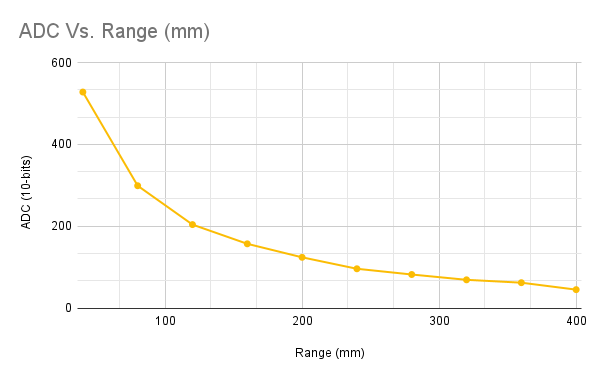
\includegraphics[ width = 0.8\linewidth]{images/ADCxRange.png}
    \caption{Gráfico com os pontos levantados experimentalmente com o programa de calibração.}
\end{figure}

%-------------------------------------------------------------
\section{Equação de conversão de valor do A/D para mm}
%Apresentação da equação de conversão de valor do A/D para mm para o sensor proximidade Sharp.
Baseado em \cite{Acroname_2013} temos que a equação final para a conversão da saída do conversor A/D (ADC) para a distância medida (R) é:

\begin{equation}
    R = \frac{m'}{(ADC+b')} - k
\end{equation}

Com os dados experimentais calculados chegamos aos valores finais.

\begin{align*}
    m'& = 32200\\
    b'& = 12\\
    k& = 15\\
\end{align*}

Então finalmente temos que a equação que transforma os valores do conversor A/D em medidas de distância em mm é:

\begin{equation*}
    R = \frac{32200}{(ADC+12)} - 15
\end{equation*}

%-------------------------------------------------------------
\newpage
\section{Código fonte}

\subsection{Calibração}

\inputminted{c}{code/NearCalibration.c}
\newpage
\subsection{Conversão e display}
\inputminted{c}{code/DataDisplay.c}
\newpage
\bibliography{references}

\end{document}